\documentclass[12pt]{article}

% Packages
\usepackage{amsmath, amssymb}
\usepackage{graphicx}
\usepackage{booktabs}
\usepackage{float}
\usepackage{geometry}
\geometry{margin=1in}
\usepackage{setspace}
\onehalfspacing

\begin{document}
\section*{Introduction}

Survival analysis provides a framework for analyzing time-to-event data in the presence of censoring. In this study, we investigate survival outcomes of patients with nasopharyngeal cancer using nonparametric methods. The primary objective is to examine how survival differs across disease stages at diagnosis.

We take on the Kaplan-Meier estimator to construct survival curves and summarize group-specific survival patterns. To complement these estimates, we report survival quantiles and restricted mean survival time (RMST), which remains well-defined under heavy censoring. Finally, we apply the log-rank test to formally assess whether survival distributions differ across stage categories.
\section*{Nonparametric Survival Analysis}

We focus on $Stage$ as the primary categorical variable, with three ordered levels: Distant, Localized, and Regional. Observations with $Unknown$ stage are excluded because they do not represent a meaningful clinical category but rather missing information.

\subsection*{Part A: Nonparametric estimation of the survival function}

For each stage group separately, we estimated the survival function nonparametrically using the Kaplan-Meier (K-M) estimator. The K-M method was selected because it is a robust handler of right censoring. It ensures that censored individuals still contribute to the survival estimate until their last known contact point. The K-M estimator is
\[
\hat{S}(t) = \prod_{j: Y_{(j)} \leq t} \left( \frac{r_{(j)} - d_{(j)}}{r_{(j)}} \right).
\]

This gives us a step function with jumps at the uncensored event times. At each event time $Y_{(j)}$, the estimated conditional probability of surviving past that time is $(r_{(j)} - d_{(j)})/r_{(j)}$, and the K-M estimate is the cumulative product of these probabilities. 

In all K-M fits, we used \texttt{conf.type = "log-log"}. This corresponds to forming confidence intervals for $\log(-\log S(t))$ first, and then back-transforming. This transformation is preferred because it guarantees that the resulting confidence interval for $S(t)$ stays within $[0,1]$. For large datasets, however, the difference is negligible. 

\newpage

\begin{figure}[htbp]
    \centering
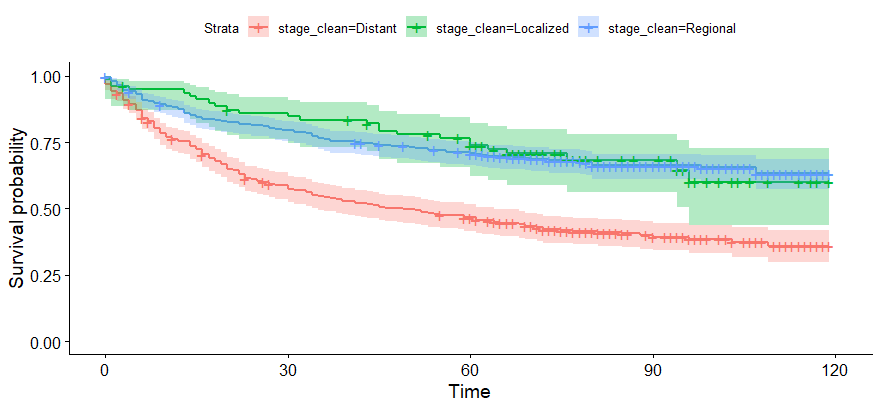
\includegraphics[width=\textwidth]{../outputs/km_curves.png}
    \caption{Kaplan-Meier Survival Curves by Stage Category}
\end{figure}

The K-M curve for "Distant" is clearly separated for the duration of 120 months. Patients staged $Localized$ and $Regional$ have higher estimated survival, and their curves remain above $0.50$ for the entire window. Patients in the $Distant$ stage have the lowest estimated survival; their curve descends rather rapidly, with a median survival of 49 months. We can visually observe heavy right censoring from the graph. Since the localized and regional stage survival curves cross, we cannot say their hazards are proportional. However, the clear deviation of the $Distant$ stage will likely prove that not all three stages are equal.

\subsection*{Part B: Quartile estimates}

\begin{table}[H]
\centering
\caption{Survival Quartiles (Months) with 95\% Log-Log Confidence Intervals}
\label{tab:quartiles_stage}
\begin{tabular}{@{}lccc@{}}
\toprule
\textbf{Stage Category} & \textbf{Q1 (75\% Survival)} & \textbf{Median (50\%)} & \textbf{Q3 (25\% Survival)} \\ \midrule
Distant   & 14 [9, 16]  & 49 [34, 64] & NA \\
Localized & 60 [30, 96] & NA          & NA \\
Regional  & 41 [31, 60] & NA          & NA \\
\bottomrule
\end{tabular}
\end{table}

Here, NA indicates that the K-M estimate does not fall below the relevant probability threshold within the observed follow-up window. The median cannot be estimated when heavy right censoring leaves the survival curve above 0.50 at the maximum observed time. This is not an error but an informative finding. Because some quartiles are non-estimable, it is helpful to calculate the restricted mean survival time (RMST). Defining $\tau$ as the maximum observed time in the data, the RMST is
\[
\hat{\mu}_{\tau} = \int_0^{\tau} \hat{S}(t)\,dt.
\]

This corresponds to the area under the K-M curve up to $\tau$, and it is always estimable regardless of the extent of right censoring. We should mention that it is biased towards tail behavior. Table~\ref{tab:rmst} reports the RMST estimates for each stage group.

\begin{table}[htbp]
\centering
\small
\begin{tabular}{lcc}
\toprule
Stage Category & RMST (months) & Std. error \\
\midrule
Distant   & 61.3 & 2.53 \\
Localized & 90.4 & 4.82 \\
Regional  & 87.6 & 2.24 \\
\bottomrule
\end{tabular}
\caption{Restricted mean survival time (RMST) by stage group.}
\label{tab:rmst}
\end{table}

The RMST values demonstrate a similar pattern to the observed quartiles; the $Distant$ stage has a lower RMST of 61.3, while the $Localized$ and $Regional$ stages are hard to distinguish, with RMST values of 90.4 and 87.6, respectively.

\subsection*{Part C: Formal test of equality of survival curves}

\paragraph{Hypothesis.}
We test
\[
H_0: S_{\text{Distant}}(t) = S_{\text{Localized}}(t) = S_{\text{Regional}}(t) \quad \text{for all } t>0,
\]
against the alternative that at least one group has a different survival function. 

We apply the log-rank test ($\rho = 0$), implemented via \texttt{survdiff(Surv(surv\_months, event) \textasciitilde{} stage\_clean, rho = 0)}. Within the Fleming-Harrington family of weighted log-rank tests, the case $\rho = \gamma = 0$ gives equal weighting over time. Our aim is to investigate whether the total cumulative survival experience of patients from different stages differs significantly; therefore, no adjusted weight on early or late stages is required. 

The log-rank test statistic is based on the vector $U$, where
\[
U = \sum w(Y_{(j)})(O_j - E_j).
\]
For the standard log-rank test, the weight function is uniformly set to $w(Y_{(j)}) = 1$. We evaluate the standardized test statistic
\[
Z = \frac{U}{\sqrt{\text{Var}(U)}},
\]
which approximates a standard normal distribution $\mathcal{N}(0, 1)$ for large sample sizes. In R, this is executed using the \texttt{survdiff()} function. A p-value below the chosen significance level (0.05) allows us to reject $H_0$, concluding a significant difference between the survival curves.

\begin{table}[htbp]
\centering
\begin{tabular}{lcccc}
\toprule
\textbf{Stage Category} & \textbf{N} & \textbf{Observed (O)} & \textbf{Expected (E)} & \textbf{$(O-E)^2/V$} \\ \midrule
Distant   & 391 & 229 & 151.0 & 66.36 \\
Localized & 79  & 25  & 38.7  & 5.44  \\
Regional  & 422 & 140 & 204.3 & 42.64 \\
\bottomrule
\end{tabular}
\caption{Log-rank test results comparing survival by stage category.}
\end{table}

The test resulted in a chi-square statistic of $\chi^2 = 66.4$ on 2 degrees of freedom, with a p-value of $p < 4 \times 10^{-15}$. 

Since the p-value is below our threshold of 0.05, we reject the null hypothesis, and there is evidence that survival times differ significantly by stage category based on the log-rank test. Specifically, the $Distant$ group experienced around 1.5 times the number of deaths expected under the null (229 observed, 151 expected), while the $Localized$ and $Regional$ groups observed fewer deaths than expected.
\section*{Conclusion}

The analysis demonstrates clear differences in survival across stage categories. Patients diagnosed at the distant stage exhibit substantially worse survival outcomes compared to those with localized or regional disease. While median survival is only estimable for the distant group due to censoring, RMST provides a consistent summary measure and confirms the same ordering of survival across groups.

The log-rank test strongly rejects the null hypothesis of equal survival functions, providing statistical evidence that stage at diagnosis is a significant determinant of survival. Overall, the results highlight the importance of early detection, as patients diagnosed at earlier stages experience markedly improved survival outcomes.
\end{document}